\section{Spherical conformal telegrapher follow-up}
\label{sec:telegraph}
The unresolved front in Fig.~\ref{fig:front} motivates a separate modification of the lapse gauge. This follow-up retains the full two-ended wormhole chart, the metric-derived elliptic shift, and independently evolved Z4c fields. It does not use the retained-domain transfer of the preceding section. In particular, neither the region inside the apparent horizon nor a neighborhood of the puncture is excised. The new numerical evidence is reported separately from the historical source and boundary trials.

\subsection{Relaxation equation and spherical coupling}
Set $D=\partial_t-\beta\partial_r$ and retain $u=\alpha-A$. We introduce a radial auxiliary component $B$ and a fixed taper $\varpi(r)$, with additions
\begin{align}
 \Delta(D\alpha)&=\chi\left[\varpi B_r+
 \left(\varpi_r+\frac{2\varpi}{r}\right)B\right],
 \label{eq:telegraph-alpha}\\
 \tau_T DB&=\kappa_T\varpi u_r-B.
 \label{eq:telegraph-B}
\end{align}
Here $B$ is unrelated to a shift-driver variable, and $\tau_T$ is unrelated to the endpoint penalty coefficient in Eq.~\eqref{eq:penalty}. The lapse addition equals $\chi r^{-2}\partial_r(r^2\varpi B)$. Its two angular terms follow from the flat-reference contraction of $B_i=B(r)x_i/r$. We retain componentwise advection of $B$ and divide Eq.~\eqref{eq:telegraph-alpha} by the total positive $\alpha$ when updating the logarithmic lapse variable. This is an explicit conformal coordinate gauge inspired by a telegrapher relaxation mechanism; it is not a covariant transformation of the Cartesian physical-lapse implementation. No Hamiltonian, momentum, or Z4 constraint is substituted into these equations.

The initial data have $B=0$. The selected taper is one for $r\leq0.56$, decreases smoothly to zero over $0.56<r<0.8$, and is zero for $r\geq0.8$. The transition uses the $C^7$ rational ramp $R_7(z)=z^8/[z^8+(1-z)^8]$, with $z=(0.8-r)/0.24$ clipped to $[0,1]$. This differs from the polynomial smoothstep used for the numerical grid map below. Consequently the direct addition vanishes near scri, preserving the existing clock and compatibility equations. An earlier version also set the coupling to zero in an inner collar; it lost effectiveness when the front entered that collar and is not the selected prescription.

Keeping $\varpi=1$ near the asymptotically flat end is regular. With $\chi=X_0r^4+O(r^5)$, $\alpha=a_2r^2+O(r^3)$, $\beta=b_1r+O(r^2)$, and $B=b_Br+O(r^2)$, Eq.~\eqref{eq:telegraph-B} gives
\begin{equation}
 \dot b_B=b_1b_B+\frac{\kappa_T(2a_2-1)-b_B}{\tau_T}.
\end{equation}
The added lapse rate is $3X_0b_Br^4+O(r^5)$, and the added logarithmic rate is $(3X_0b_B/a_2)r^2+O(r^3)$. Thus the leading AF lapse coefficient equation is unchanged. The endpoint condition $B(0)=0$ is preserved by its evolution; this argument uses AF asymptotics, not regular-center reflection parity.

\subsection{Characteristic speeds and the meaning of compression}
The frozen radial lapse--trace--flux subsystem has speeds
\begin{equation}
 c_0=-\beta,\qquad
 c_\pm=-\beta\pm\sqrt{\chi\left(F+\frac{\kappa_T\varpi^2}{\tau_T}\right)}.
\label{eq:telegraph-speeds}
\end{equation}
The shift and metric factors are essential. Using the isolated telegrapher speed alone would underestimate the coupled propagation speed. Define $c_g^2=\chi F$ and $c_T^2=\chi\kappa_T\varpi^2/\tau_T$. In the locally advected frame, the frozen Fourier dispersion polynomial is
\begin{equation}
 s^3+\frac{s^2}{\tau_T}+(c_g^2+c_T^2)k^2s
 +\frac{c_g^2k^2}{\tau_T}=0.
\label{eq:telegraph-dispersion}
\end{equation}
For nonzero $k$, positive $c_g^2,c_T^2$, and $\tau_T>0$, the Routh--Hurwitz inequality is strict. The high-frequency propagating pair has damping rate
\begin{equation}
 \gamma_\infty=\frac{c_T^2}{2\tau_T(c_g^2+c_T^2)}.
\end{equation}
These frozen-subsystem statements motivate the mechanism; they do not prove stability or shock avoidance for the nonlinear free-Z4c system with elliptic shift feedback.

For each family we evolve a ray position and a ray-map Jacobian $\mathcal J_\pm$,
\begin{equation}
 \dot r_\pm=c_\pm(t,r_\pm),\qquad
 \frac{\dd}{\dd t}\log\mathcal J_\pm=\partial_r c_\pm(t,r_\pm).
\label{eq:telegraph-rays}
\end{equation}
There are 81 matched seeds per family, uniformly spanning $0.12\leq r\leq0.4$, activated exactly at $t=1$. The stage geometry and stage elliptic shift supply the speed at every RK evaluation. A shape-preserving $C^1$ piecewise cubic Hermite interpolant supplies both the speed and its analytic derivative\cite{PCHIP}; it is applied only to passive diagnostics and cannot smooth the evolved lapse. Boundary exits are located using a continuous RK4 extension\cite{RK4Dense}; the terminal position and compression are evaluated at the same exit event and then frozen. The implementation also checks for an exit followed by a return within a step. Intermediate ray stages may continue the endpoint speed polynomial by at most one boundary-cell width; the geometry and elliptic equations are never evaluated outside the domain. Terminal coincidences at scri are not characteristic crossings.

For a regular Lipschitz finite-grid velocity, $\mathcal J=\exp(\int\partial_rc\,\dd t)$ stays positive. Finite-grid ray ordering therefore cannot prove continuum noncrossing. Conversely, a very small positive $\mathcal J$ is compression, not an observed intersection. The relevant evidence is joint spatial and temporal convergence of the lapse, its gradient, the constraints, and the ray diagnostics. The original unmodified gauge gave inward $\min\mathcal J$ at $t=3$ of $1.26\times10^{-5}$ and $1.22\times10^{-8}$ at $N=513$ and $1025$, respectively. This resolution-dependent compression supports the unresolved-steepening diagnosis, without importing a shock theorem from a simpler slicing system\cite{Alcubierre2005}.

\subsection{Mapped discretization and implementation checks}
The baseline is the modified logarithmic source of Eq.~\eqref{eq:physical-log}, with constant constraint damping. The selected parameters are $M=1/3$, $\nu=1$, $\kappa_T=0.005$, $\tau_T=0.02$, and $\Delta t=0.05\Delta x$, with $x_i=i/(N-1)$. All continuum equations remain expressed in $r$. A fixed numerical map resolves the shrinking inner layer:
\begin{equation}
 E(x)=\frac{\operatorname{expm1}(32x)}{2\operatorname{expm1}(16)}.
\end{equation}
It is used through $x=0.3$, joined to $r=x$ over $0.3<x<0.5$ by $r=(1-S)E+Sx$, and followed by the identity through $x=0.8$. For the inner join, $S=S_7((x-0.3)/0.2)$, where
\begin{equation}
 S_7(z)=\sum_{j=8}^{15}\binom{15}{j}z^j(1-z)^{15-j},
 \qquad 0\leq z\leq1.
\end{equation}
For $x>0.8$, let $L=0.2$ and $y=(x-0.8)/L$ and use
\begin{equation}
 r=x+\tfrac12Ly^8(1-y),\qquad
 J_x\equiv\frac{\dd r}{\dd x}=1+\tfrac12y^7(8-9y).
\end{equation}
This join is $C^7$, monotone, fixes actual scri, and gives $J_x(1)=1/2$. It refines the outer endpoint without changing the inner map. Derivative and interval-quadrature weights are constructed on the actual $r_i$; the endpoint penalty spacing is $\Delta xJ_x(1)$. The map is fixed across resolution, and no physical nodes are removed.

The selected implementation retains seven-point derivative stencils and seven-point shift quadrature. It replaces sixth-difference dissipation by eighth-difference dissipation. Writing $D_p$ for the unscaled $p$th forward difference, the mapped filter is
\begin{align}
 Q_{2p}&=-\frac{\epsilon}{2^{2p}\Delta x}
 J_x^{-1}D_p^T\operatorname{diag}(W\overline J)D_p,\\
 \overline J_i&=\frac{p+1}{\sum_{j=0}^{p}1/J_{x,i+j}},\qquad p=4,
\end{align}
with $\epsilon=0.5$ and the existing nonnegative physical-radius taper $W$. The AF coefficient column is excluded from this filter, while its continuum endpoint ODE is still evolved. Geometry and $B$ use the same filter. Its discrete $J_x$-weighted energy contribution is nonpositive and its smooth interior truncation contribution is $O(\Delta x^7)$. The isolated-filter guard is $\Delta t\epsilon/\Delta x\leq2/(p+1)$; characteristic and relaxation guards are also enforced. These properties do not provide a stability estimate for the combined nonlinear operator.

On this map, the full-grid constraint RMS is
\begin{equation}
 \normr{C}=\left[\frac{\sum_i r_i^2J_{x,i}C_i^2}
 {\sum_i r_i^2J_{x,i}}\right]^{1/2}.
\label{eq:telegraph-norm}
\end{equation}
It uses the implemented conformal constraint quantities and is not a proper-volume norm. It downweights the near-puncture region and gives zero weight to the endpoint $r=0$, so we also retain unweighted pointwise maxima on the full grid and on $0\leq r<0.8$. The latter cutoff removes the outer region toward scri, not the black-hole interior. No differential constraint is projected, reset, or masked in the acceptance assessment.

The implementation checks include independent nonzero-flux Python/compiled rates, spherical angular contractions, free-constraint RK stages, exact zero-flux regression, mapped differentiation/quadrature, filter energy identities, stage rays, and compensated-state restart. The complete 55-group suite passed after the dense-exit implementation. A subsequent analysis-only change passed its two targeted CTest groups; it is not described as a rerun of the expanded 56-group suite. Pure exit-event oracles showed approximately fourth-order errors, whereas the actual $C^1$ interpolated speed requires its own measured timestep study.

\subsection{Completed spatial experiment and measured limitations}
\newcommand{\TeleBulkOrder}{5.89}
\newcommand{\TeleEndpointOrder}{5.63}
\newcommand{\TeleHOrder}{6.52}
\newcommand{\TeleMOrder}{6.48}
\newcommand{\TeleThetaOrder}{6.62}
\newcommand{\TeleZOrder}{6.49}
\newcommand{\TeleGradientPercent}{0.103}
\newcommand{\TeleSpatialAssessment}{All listed spatial, boundary, and positivity checks pass for this fixed candidate. This is a finite-duration spatial result, not completion of the independent-control protocol.}
\newcommand{\TeleFinalHMax}{\ensuremath{2.290\times10^{-5}}}
\newcommand{\TeleFinalHRadius}{\ensuremath{1.465\times10^{-6}}}
\newcommand{\TeleAHMassError}{\ensuremath{1.267\times10^{-10}}}
\newcommand{\TeleRayGap}{\ensuremath{8.323\times10^{-11}}}
\newcommand{\TeleRayPositionError}{\ensuremath{6.209\times10^{-9}}}
\newcommand{\TeleRayLogError}{\ensuremath{5.507\times10^{-6}}}
\newcommand{\TeleMSMassError}{\ensuremath{1.476\times10^{-4}}}
\newcommand{\TeleAFMassError}{\ensuremath{2.916\times10^{-6}}}
\newcommand{\TeleMinLogJ}{-17.554446}
\newcommand{\TeleRayPositionOrder}{4.72}
\newcommand{\TeleRayLogOrder}{3.59}

The three related grids $N=1025,2049,4097$ reach $t=10$ with identical continuum parameters, numerical map, CFL factor, derivative width, and dissipation amplitude. This includes the complete initial transient and late inward compression. The comparison uses exact common physical nodes and 201 saved times; the constraint and boundary maxima in Table~\ref{tab:telegraph} are accumulated over every accepted state or every checked stage, as appropriate, rather than inferred only from those snapshots.

\begin{table}[tbp]
\caption{Full-duration telegrapher results on $0\leq t\leq10$. The Hamiltonian columns are maxima over accepted states; the pole column is the maximum checked scri residue. The pointwise Hamiltonian column includes $0\leq r<0.8$, retaining the puncture neighborhood.}
\label{tab:telegraph}
\begin{ruledtabular}
\small
\setlength{\tabcolsep}{3pt}
\begin{tabular}{rccc}
$N$ & $\max_t\normr{\HH}$ & $\max_{t,r<0.8}|\HH|$ & Scri pole\\
\hline
1025 & $5.401\times10^{-5}$ & $8.121\times10^{-2}$ & $2.833\times10^{-6}$\\
2049 & $1.405\times10^{-6}$ & $2.238\times10^{-3}$ & $1.414\times10^{-7}$\\
4097 & $1.528\times10^{-8}$ & $2.290\times10^{-5}$ & $4.212\times10^{-9}$

\end{tabular}
\end{ruledtabular}
\end{table}

The peak-in-time field-difference orders are \TeleBulkOrder\ in the bulk and \TeleEndpointOrder\ near scri. The finest-pair orders of the accepted-state RMS maxima for $(\HH,\MM,\Th,Z_r)$ are $(\TeleHOrder,\TeleMOrder,\TeleThetaOrder,\TeleZOrder)$. The maximum matched lapse-gradient discrepancy, normalized separately at each time by the fine-grid peak on common nodes, is \TeleGradientPercent\ percent. The original thresholds are unchanged: bulk field and constraint order at least $3.5$, endpoint field order at least $3$, finest Hamiltonian RMS below $10^{-5}$, pointwise Hamiltonian below $10^{-3}$ on $r<0.8$, and matched gradient discrepancy below $10\%$. \TeleSpatialAssessment

Figures~\ref{fig:tele-lapse} and \ref{fig:tele-resolution} show that an inward-moving nonmonotone lapse structure remains. Its survival as a profile feature is not itself a convergence failure: the relevant questions are whether its amplitude, width, derivatives, and associated constraints stabilize under refinement. Conversely, close agreement of two lapse curves alone is insufficient. By $t=10$ the physical-lapse structure occupies radii of order $10^{-6}$, which motivates the fixed exponential grid. A large coordinate derivative in this shrinking region is not, by itself, proof of a continuum discontinuity.

\begin{figure*}[tp]
 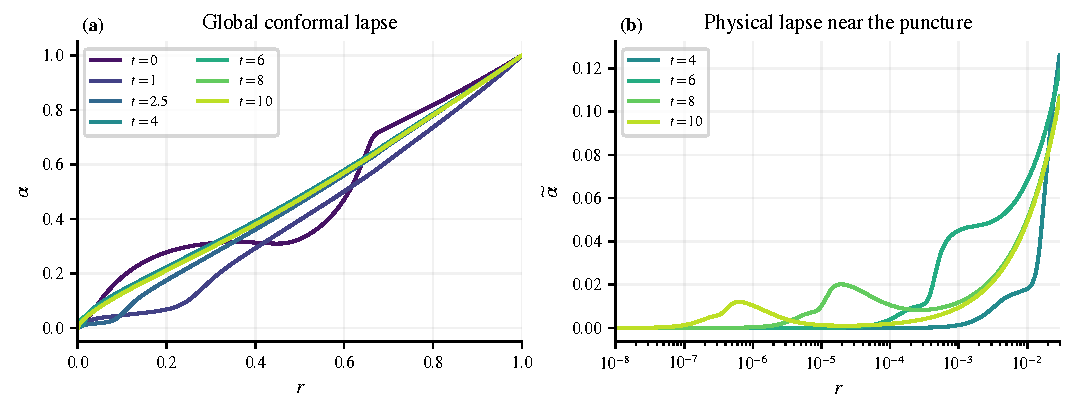
\includegraphics[width=\textwidth]{telegraph_lapse_evolution}
 \caption{Telegrapher lapse evolution on the finest completed grid, $N=4097$. The global panel uses conformal $\alpha$, which remains finite at scri. The inner panel uses physical $\widetilde\alpha=\alpha/\Omega$ and logarithmic radius to expose the late nonmonotone structure. Curves use saved profiles without smoothing or temporal interpolation. The remaining bump is not declared eliminated.}
 \label{fig:tele-lapse}
\end{figure*}
\begin{figure*}[tp]
 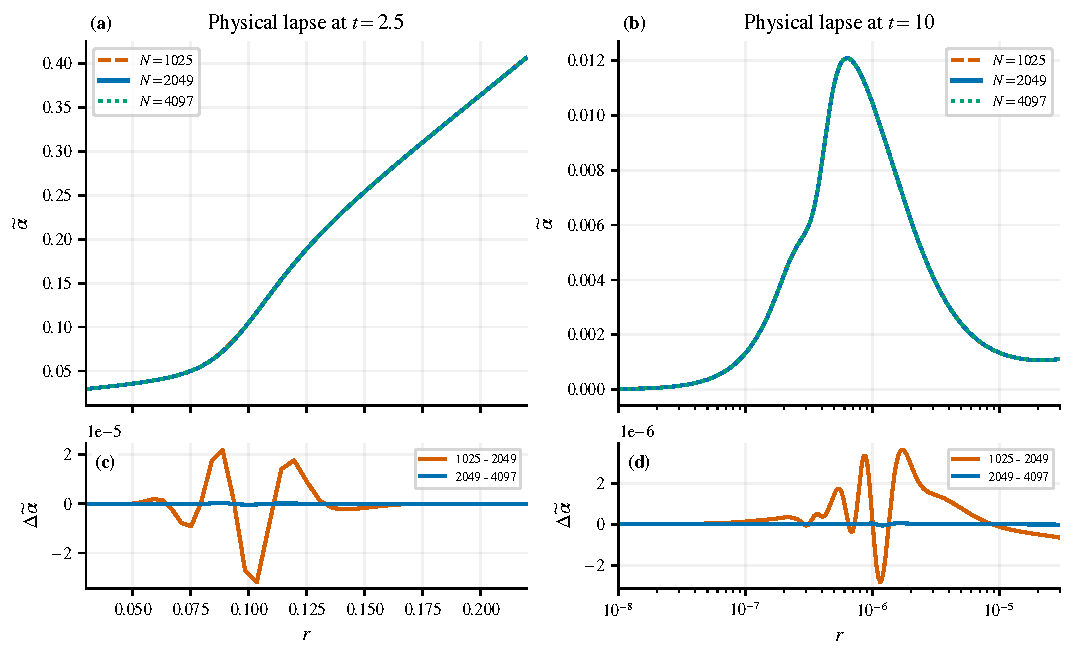
\includegraphics[width=\textwidth]{telegraph_lapse_resolution}
 \caption{Three-grid physical-lapse comparison at $t=2.5$ and $t=10$. The lower panels show raw consecutive-grid differences at matching physical nodes. The late panel retains the near-puncture structure instead of cutting it out. These are profile comparisons; whole-trajectory derivative and constraint checks are reported separately.}
 \label{fig:tele-resolution}
\end{figure*}

Figure~\ref{fig:tele-constraints} presents all four constraint histories. The radial RMS can be small while a sharply localized inner error is appreciable. At $t=10$ on $N=2049$, for example, $\normr{\HH}=9.67\times10^{-8}$ but $\max_r|\HH|=2.24\times10^{-3}$. That peak lies at $r=1.46\times10^{-6}$, well inside the apparent horizon at $r=0.10765$; the exterior maximum is $1.05\times10^{-7}$. This is a localization diagnostic, not an exterior-only acceptance rule. On the finest grid, the corresponding final full-grid maximum is \TeleFinalHMax\ at $r=\TeleFinalHRadius$, and the peak sampled apparent-horizon mass error over the full run is \TeleAHMassError. The maximum sampled finite-node Misner--Sharp mass discrepancy over the same trajectory is \TeleMSMassError, including the near-scri and inner nodes; the maximum sampled AF-end coefficient-mass discrepancy is \TeleAFMassError. The actual scri mass slot is undefined in this diagnostic and is not included in that finite-node maximum. Neither small exterior error nor accurate horizon mass overrides an inner constraint failure. Figure~\ref{fig:tele-inner} makes the pointwise error, growing lapse gradient, error location, and mass diagnostic visible together.

\begin{figure*}[tp]
 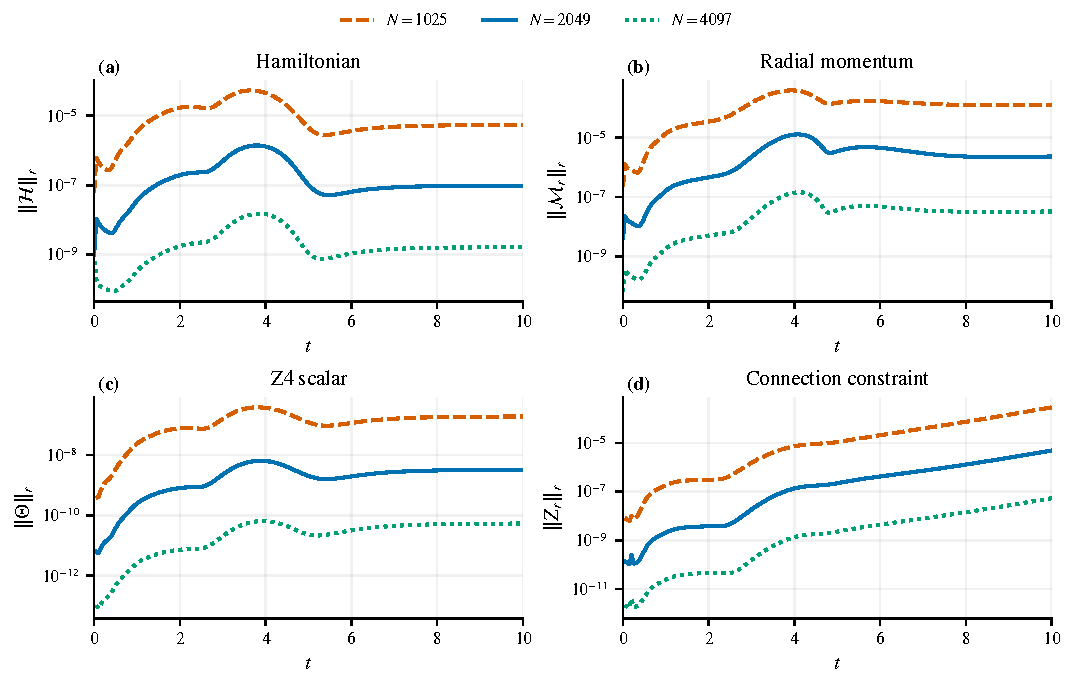
\includegraphics[width=\textwidth]{telegraph_constraints}
 \caption{Full-domain radial RMS constraints for the completed telegrapher sequence, using Eq.~\eqref{eq:telegraph-norm}. Every plotted value was recomputed from saved fields and checked against the recorded history. These curves sample every $0.05$ time units; the accepted-state maxima in Table~\ref{tab:telegraph} can be slightly larger. No interior mask is applied. The radial weighting suppresses small-radius contributions, so Fig.~\ref{fig:tele-inner} also reports the full-grid pointwise Hamiltonian error.}
 \label{fig:tele-constraints}
\end{figure*}
\begin{figure*}[tp]
 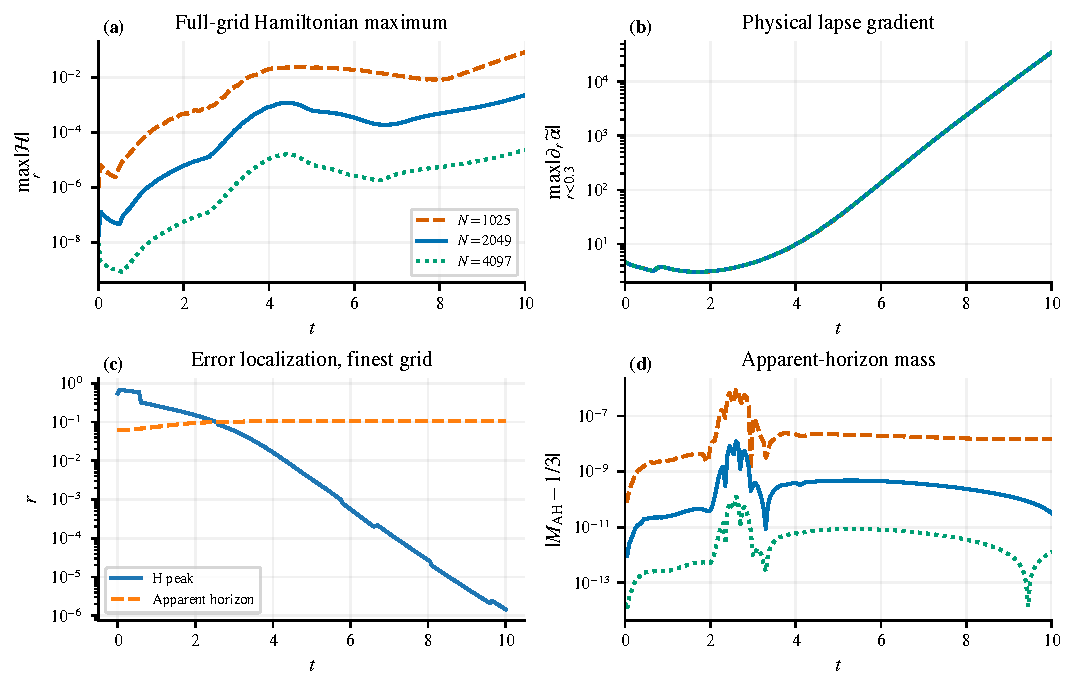
\includegraphics[width=\textwidth]{telegraph_inner_errors}
 \caption{Diagnostics that prevent a small radial RMS from hiding the inward layer. (a) Unweighted full-grid Hamiltonian maximum. (b) Physical-lapse gradient over $0\leq r<0.3$, evaluated with analytic AF factors and seven-point chart derivatives. (c) Position of the finest-grid Hamiltonian peak compared with the apparent horizon. (d) Independent apparent-horizon mass error. The horizon is identified from the outgoing expansion; this does not locate the event horizon. Mass errors near floating-point precision do not establish an asymptotic order.}
 \label{fig:tele-inner}
\end{figure*}

The tracked rays retain their ordering in the sampled spatial comparison. At $t=10$, all 81 inward rays remain active and all 81 outward rays have exited at scri. The finest minimum active inward $\log\mathcal J_-$ is \TeleMinLogJ, and the minimum active neighboring-ray separation is \TeleRayGap. The maximum middle-to-fine differences over the full trajectory are \TeleRayPositionError\ in ray position and \TeleRayLogError\ in $\log\mathcal J$, including terminal states. The observed peak-difference orders are \TeleRayPositionOrder\ and \TeleRayLogOrder, respectively. Figure~\ref{fig:tele-rays} shows the ray fans, compression, and refinement differences. These measurements describe strongly compressed finite-grid characteristics; they do not establish a continuum intersection or its absence.

\begin{figure*}[tp]
 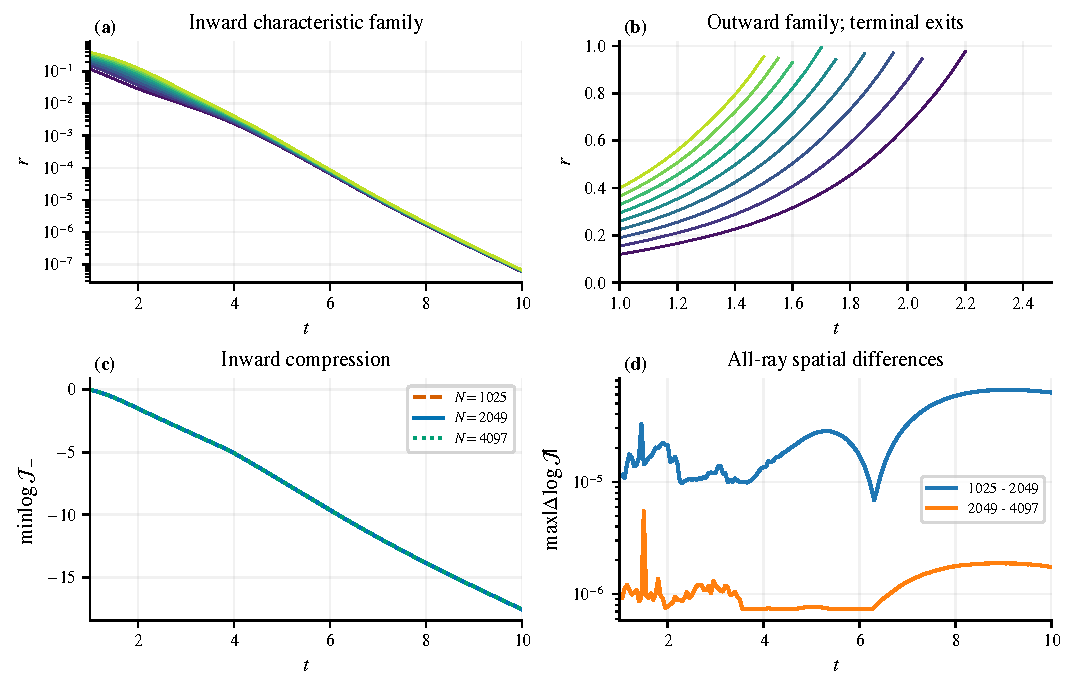
\includegraphics[width=\textwidth]{telegraph_characteristics}
 \caption{RK-stage characteristic tracking with matched dense exit events. The upper panels show nine representative seeds from each of the 81-ray families on $N=4097$. The outward panel zooms to the exit interval. Paths end at the last saved active point; no precise event time is fabricated from the plotting cadence. The lower-left panel shows inward compression across resolutions. The lower-right comparison includes all rays, including their frozen terminal compression. Positive finite-grid Jacobians and ordered rays are not a continuum shock-avoidance proof.}
 \label{fig:tele-rays}
\end{figure*}

\subsection{Independent timestep evidence at the stopping point}
The baseline and independent half-step $N=2049$ trajectories both reach $t=10$. The quarter-step control was paused at the requested finest-grid stopping point, with saved reports through $t=8.35$. Consequently the required full-duration three-level temporal-order and timestep-to-spatial-error assessment remains incomplete. The completed baseline--half-step comparison gives maximum bulk and endpoint field differences of $4.04\times10^{-12}$ and $2.33\times10^{-12}$, a Hamiltonian pointwise difference of $5.71\times10^{-10}$, and ray-position and $\log\mathcal J$ differences of $4.27\times10^{-13}$ and $7.68\times10^{-8}$. Two timestep levels alone do not establish temporal order. These raw differences, and the earlier short diagnostic pilot, cannot replace the missing robustness controls.



\subsection{Long-duration puncture pilot: exterior accuracy and termination}
\label{sec:tele-long}
A separate low-resolution continuation targeted $t=500$ on $N=1025$, starting from the verified $t=10$ checkpoint of the genuine wormhole trajectory. The frozen numerical source, binaries, map, CFL factor, relaxation parameters, and full-domain boundary treatment were unchanged. The run stopped at $t=43.836474609375$ with the native error \code{g=1 gauge or positivity violation}. Figure~\ref{fig:tele-long} reports all validated saved states through $t=43.8$, including the parent trajectory. The requested duration was not reached. This is a single-grid survival pilot, not an additional convergence study.

For this long-duration pilot we assess an apparent-horizon-exterior error budget and take apparent-horizon mass conservation as the primary invariant check. At each saved time, let $E(t)=\{i:r_i\geq r_{\rm AH}(t)\}$, where the existing outgoing-expansion finder locates $r_{\rm AH}$. With the same mapped radial weights $w_i=r_i^2(\dd r/\dd x)_i$ used previously, define
\begin{equation}
 \|C\|_{r,E}^2=\frac{\sum_{i\in E(t)}w_i C_i^2}{\sum_{i\in E(t)}w_i},
 \qquad C\in\{\HH,\MM,\Th,Z_r\}.
 \label{eq:exterior-norm}
\end{equation}
The pointwise budget uses $\max_{i\in E(t)}|C_i|$. Interior errors and puncture-end mass estimates are excluded from this budget. The normalization uses only exterior weights, rather than filling the excluded interior with zeros. This is a diagnostic selection: the evolution still includes every puncture-interior node. The historical three-grid full-domain assessment through $t=10$ remains unchanged and is labeled separately.

At the last saved time $t=43.8$, the exterior RMS values for $(\HH,\MM,\Th,Z_r)$ are $(1.79\times10^{-7},2.44\times10^{-6},5.00\times10^{-8},5.21\times10^{-7})$. The exterior Hamiltonian maximum is $5.88\times10^{-6}$. These late values remain nearly unchanged from $t=10$. The initial transient remains in the budget: the maximum sampled exterior Hamiltonian and momentum RMS values on $0\leq t\leq43.8$ are $1.84\times10^{-5}$ and $4.92\times10^{-5}$. The apparent-horizon mass error is $3.93\times10^{-8}$ at $t=43.8$, or $1.18\times10^{-7}$ relative to $M=1/3$; its peak sampled absolute error over the whole interval is $8.79\times10^{-7}$, corresponding to relative error $2.64\times10^{-6}$. The late mass error grows gradually while remaining below the initial-transient peak.

The saved exterior diagnostics do not show a blow-up before termination. Nevertheless, excluding interior diagnostic errors does not disable the full-domain evolution guard. The termination checkpoint remains finite, its metric deviation is exactly zero, and reconstructed lapse and conformal factor are positive at positive-radius nodes. The generic guard message does not preserve the offending stage or radial index. An offline replay, described below, localizes the failure to lapse underflow at the second positive-radius node during RK stage four. Puncture-interior constraints and mass estimates remain archived diagnostics and are excluded from the exterior budget. The result supports preserved horizon mass and a nearly steady late exterior constraint budget through the last saved profile, but does not establish survival to $t=500$ or exterior convergence. The failed trajectory is retained; the following floor controls are separate experiments.

\begin{figure*}[tp]
 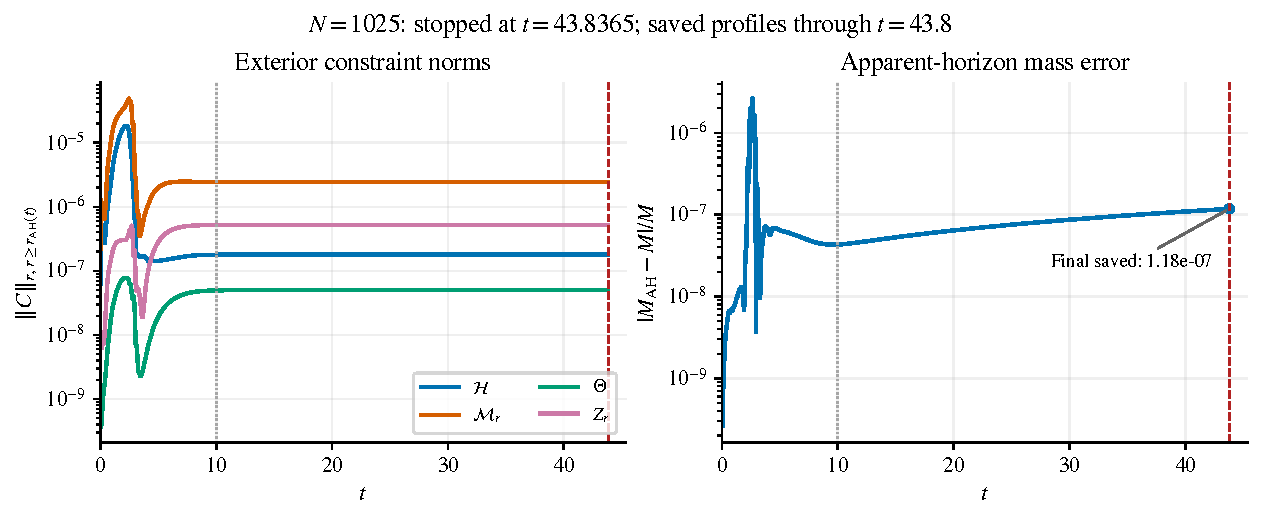
\includegraphics[width=\textwidth]{telegraph_long_exterior_status}
 \caption{Final saved history of the $N=1025$ puncture continuation targeting $t=500$. Left: apparent-horizon-exterior radial RMS constraints, normalized over the exterior region at each saved time. Right: relative apparent-horizon mass error, the primary invariant in the revised long-run budget. The gray dotted line marks the verified restart at $t=10$; the red dashed line marks the native guard stop at $t=43.8365$. Curves end at the last saved time $t=43.8$ and are not extrapolated to the failed stage. Puncture-interior errors and puncture mass estimates do not enter this budget. All 877 distinct saved profiles were checked for finite fields, reconstructed full-domain norms, and independently recomputed apparent horizons before evaluating the exterior diagnostics.}
 \label{fig:tele-long}
\end{figure*}


\subsection{Localized lapse underflow and a configurable floor}
\label{sec:lapse-floor}
Replaying the failed step on an isolated checkpoint copy with its frozen kernels reproduces the native rejection without advancing the original trajectory. At the second positive-radius node, $r=3.63\times10^{-9}$, the conformal lapse falls from $5.20\times10^{-11}$ at stage one to $1.25\times10^{-11}$ and $1.37\times10^{-13}$ at stages two and three. The fourth-stage value has $\log\alpha=-1109.3$, so reconstruction underflows to zero. The metric deviation remains zero and the conformal factor remains positive. The telegrapher contribution to the logarithmic lapse rate is approximately $-5.87\times10^4$, $-2.44\times10^5$, and $-2.22\times10^7$ in the first three stages, whereas the base-gauge contribution is positive and only of order $10^2$. Thus the additive flux contribution divided by the collapsing lapse drives the immediate rejection. Figure~\ref{fig:lapse-stop} shows the increasingly irregular inner profile and the replayed stage values.

We added the user-configurable input \code{lapse_floor}, with default $10^{-10}$ and $0$ to disable it. The CLI spelling is \code{--lapse-floor}. At ordinary nodes $0<r<1$, the numerical update applies
\begin{equation}
 \widetilde\alpha_i\leftarrow\max(\widetilde\alpha_i,\alpha_{\min}),
 \qquad \alpha_{\min}=10^{-10}\quad\hbox{by default},
\end{equation}
before each RK stage and after every accepted step, including initialization before the first report. The projection is implemented in the logarithmic lapse chart with an upward rounding margin. Only the clipped accepted lapse components have their compensated-update remainder reset. The AF coefficient endpoint and scri clock are unchanged; no constraint or other geometric field is projected. This is a finite-grid regularization of the unresolved interior, not an established continuum AF-end prescription. Historical inputs are explicitly pinned to zero floor, and the selected value is included in restart validation.

The native implementation with zero floor still reproduces the original rejection. With $\alpha_{\min}=10^{-10}$, a separate checkpoint control completes 20\,480 steps, one additional time unit, to $t=44.8365$. Only the first two positive-radius nodes require clipping in this control. Its final relative apparent-horizon mass error is $1.20\times10^{-7}$ and its exterior Hamiltonian RMS is $1.79\times10^{-7}$. Preliminary isolated controls with floors $10^{-8}$ and $10^{-6}$ also complete one time unit; these short controls do not establish long-duration stability. Seven targeted telegrapher test groups pass, including independent projected-RK comparison, preserved endpoint slots, disabled and invalid inputs, and exact floor-bound checkpoint restart. A separate fresh $N=1025$ wormhole trial with the default floor also targeted $t=500$. Its terminal outcome is reported below, separately from the unfloored failure and the completed three-grid study.

\begin{figure*}[tp]
 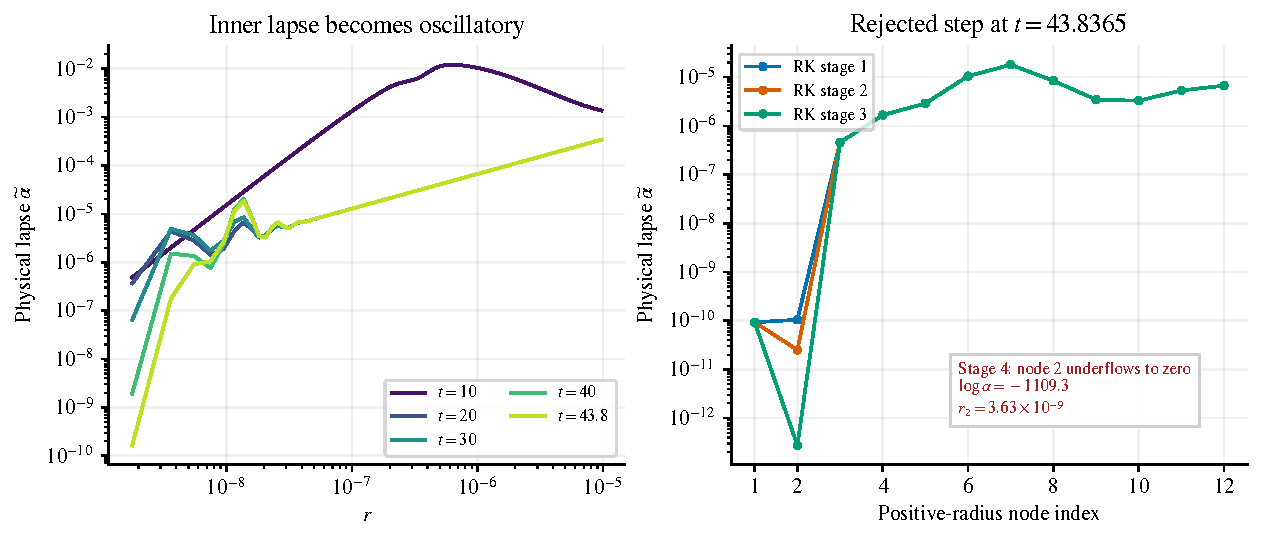
\includegraphics[width=\textwidth]{telegraph_lapse_stop}
 \caption{Diagnosis of the unfloored termination. Left: raw physical-lapse profiles in the innermost resolved region, showing irregular structure concentrated near the first few grid points. Right: the first three stages of an offline replay of the rejected step, using the frozen original kernels. Node two reaches $\log\alpha=-1109.3$ at stage four and underflows to zero; that zero is stated rather than plotted on the logarithmic axis. This local failure occurs far inside the apparent horizon. The floor controls are separate numerical experiments and do not overwrite this evidence.}
 \label{fig:lapse-stop}
\end{figure*}


\subsection{Terminal outcome of the floored duration trial}
\label{sec:floored-long}
The fresh wormhole trial with $\alpha_{\min}=10^{-10}$ stops at $t=84.798291015625$, after 1\,736\,669 accepted steps, with the native error \code{telegraph coupled-speed/relaxation timestep guard}. All 1696 saved profiles through $t=84.75$ were validated with the same source-binding, field-finiteness, full-domain-norm, and independent horizon checks used for the unfloored export. The original failed trajectory is preserved; this trial begins at $t=0$ with the floor applied to the analytic pre-collapsed lapse.

Figure~\ref{fig:floored-long} separates the exterior budget from the unresolved inner behavior. At $t=84.75$, the exterior RMS values for $(\HH,\MM,\Th,Z_r)$ are $(1.79\times10^{-7},2.44\times10^{-6},5.00\times10^{-8},5.21\times10^{-7})$, nearly unchanged from their late unfloored values. The exterior Hamiltonian maximum is $5.88\times10^{-6}$. The final saved apparent-horizon mass error is $7.01\times10^{-8}$, or $2.10\times10^{-7}$ relative to $M=1/3$. The maximum sampled relative error, $2.64\times10^{-6}$, still occurs during the initial transient. The last saved scri pole residue is $4.59\times10^{-13}$, with zero clock and nullness residuals. These statements apply to saved states, not to a successful continuation through the rejected step.

The floor remains localized far inside the apparent horizon: its outermost activation over the trajectory is $r=6.29\times10^{-7}$, compared with $r_{\rm AH}\simeq0.10765$. Nevertheless, the maximum upward correction to the stored lapse logarithm grows to $5.25\times10^3$ by the last saved state and $1.20\times10^4$ in the terminal diagnostics. This is substantial numerical clipping, rather than a uniformly small perturbation. The lower bound prevents lapse underflow but does not bound the independently evolved geometry or the elliptic shift.

An isolated replay with the exact frozen kernels reproduces the guard at the first stage of the next attempted step. The maximum occurs at positive-radius node three, $r=5.53\times10^{-9}$, where the physical lapse remains $10^{-10}$ but the reconstructed shift is $\beta^r\simeq3.93\times10^7$. Both coupled characteristic speeds are approximately $-3.93\times10^7$: shift transport dominates their splitting. With the mapped Jacobian $\dd r/\dd x=1.98\times10^{-6}$ and $\Delta t=4.8828125\times10^{-5}$, the checked mapped Courant number is $9.94\times10^{11}$, exceeding the limit $0.4$. The relaxation ratio remains $\Delta t/\tau=0.0024414$, so the speed condition triggers this guard. The last saved accumulated Courant maximum was only $0.2000$; the terminal event is not inferred by extrapolating that sampled history. The replay changes neither parameters nor timestep and does not continue the failed trajectory. Subsequent fresh repair trials are assessed separately in Sec.~\ref{sec:tele-repair-evidence}. The evidence establishes a later discrete inner failure despite a preserved saved exterior budget, not survival to $t=500$, continuum shock formation, or convergence of the floor prescription.

\begin{figure*}[tp]
 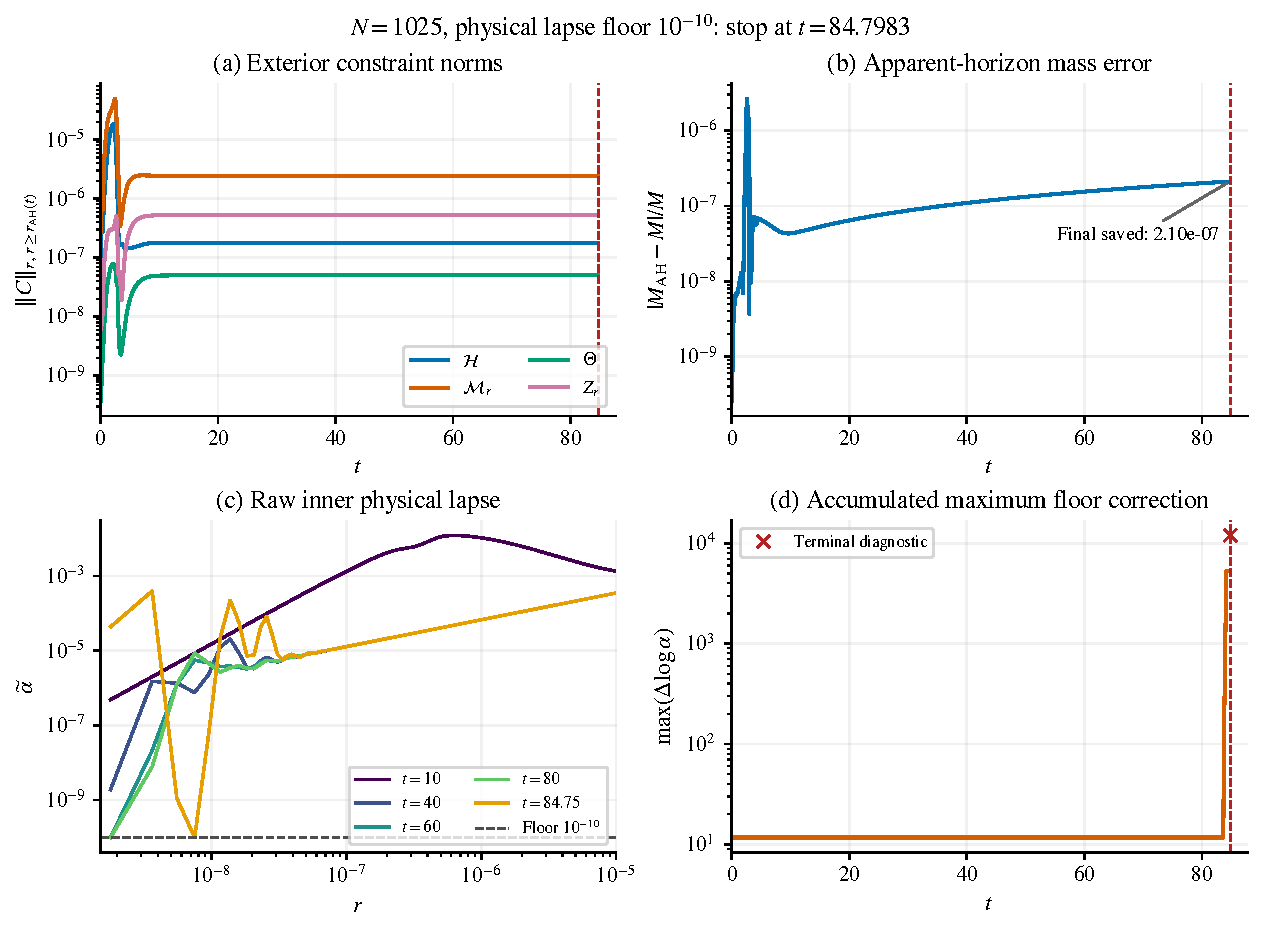
\includegraphics[width=\textwidth]{telegraph_floored_long}
 \caption{Separate fresh wormhole trial with physical lapse floor $10^{-10}$. (a) Apparent-horizon-exterior RMS constraints. (b) Relative apparent-horizon mass error. These primary diagnostics retain the complete initial transient and exclude the horizon interior. (c) Raw inner physical-lapse profiles, with the imposed floor marked; no smoothing is applied. (d) Accumulated maximum upward correction to the stored lapse logarithm, with the terminal diagnostic marked separately from the saved histories. The vertical red lines mark the speed-guard stop at $t=84.7983$; saved histories end at $t=84.75$. Large interior clipping is disclosed but is not substituted for the requested exterior error budget.}
 \label{fig:floored-long}
\end{figure*}


\subsection{Unsuccessful repairs and limits of the follow-up}
The refinement strategy was selected through documented failures. The inner-collar coupling lost influence after the front entered the collar; retaining the AF-regular coupling addressed that mechanism. Uniform and insufficiently clustered grids then underresolved the shrinking layer. A global clustering map improved inner resolution while degrading scri, motivating a map that preserves outer resolution. Increasing the differentiation width from seven to nine points produced a severe scri failure: the $N=513$, $t=6$ pilots had pole residues of order $5.6\times10^3$ and Hamiltonian RMS of order $0.20$, despite reaching their target time. A restricted outer-block spectrum supported a discrete-boundary explanation, but did not prove stability of the full system. Width seven was retained.

The previous KO6 exponential-map sequence met the inner spatial constraint magnitude and convergence gates through $t=10$ but missed the scri pole threshold: its finest residue was $1.0504\times10^{-7}$ against $10^{-7}$. Its old linear-ray/terminal-exit treatment also failed the independent compression accuracy criterion, with a timestep-to-spatial difference ratio of $0.2544$. Replacing only the speed interpolant by PCHIP did not cure terminal-event error. In the subsequent short pilot, adding matched dense exit events reduced the all-ray compression difference from $1.49\times10^{-4}$ to $9.89\times10^{-7}$ and its timestep-to-spatial ratio to $0.00168$. The saved geometry and auxiliary-flux histories were byte-identical across this diagnostic change. These were repairs to characteristic measurement, not an additional lapse-smoothing mechanism.

The current study ends at the requested finest-grid milestone. Independent shift-quadrature refinements, KO-amplitude variations, and adjacent fixed $\kappa_T,\tau_T$ three-grid controls were prepared but not executed. Their absence prevents a claim of robust parameter-independent convergence. Neither the telegrapher modification nor a successful finite-duration convergence check establishes a stationary trumpet limit, nonlinear shock avoidance for arbitrary data, or the missing scalar-collapse and radiation results.
